%%%%%%%%%%%%%%%%%%%%%%%%%%%%%%%%%%%%%%%%%
% University Assignment Title Page 
% LaTeX Template
% Version 1.0 (27/12/12)
%
% This template has been downloaded from:
% http://www.LaTeXTemplates.com
%
% Original author:
% WikiBooks (http://en.wikibooks.org/wiki/LaTeX/Title_Creation)
%
% License:
% CC BY-NC-SA 3.0 (http://creativecommons.org/licenses/by-nc-sa/3.0/)
% 
% Instructions for using this template:
% This title page is capable of being compiled as is. This is not useful for 
% including it in another document. To do this, you have two options: 
%
% 1) Copy/paste everything between \begin{document} and \end{document} 
% starting at \begin{titlepage} and paste this into another LaTeX file where you 
% want your title page.
% OR
% 2) Remove everything outside the \begin{titlepage} and \end{titlepage} and 
% move this file to the same directory as the LaTeX file you wish to add it to. 
% Then add \input{./title_page_1.tex} to your LaTeX file where you want your
% title page.
%
%%%%%%%%%%%%%%%%%%%%%%%%%%%%%%%%%%%%%%%%%
%\title{Title page with logo}
%----------------------------------------------------------------------------------------
%	PACKAGES AND OTHER DOCUMENT CONFIGURATIONS
%----------------------------------------------------------------------------------------

\documentclass[12pt]{article}
\usepackage[english]{babel}
\usepackage[utf8x]{inputenc}
\usepackage{amsmath}
\usepackage{graphicx}
\usepackage[colorinlistoftodos]{todonotes}
\usepackage{multirow}
\usepackage{enumerate}
\usepackage{subcaption}
\usepackage{tabularx}

\begin{document}

\begin{titlepage}

\newcommand{\HRule}{\rule{\linewidth}{0.5mm}} % Defines a new command for the horizontal lines, change thickness here

\center % Center everything on the page
 
%----------------------------------------------------------------------------------------
%	HEADING SECTIONS
%----------------------------------------------------------------------------------------

\textsc{\LARGE University of California, Irvine}\\[1.5cm] % Name of your university/college
\textsc{\Large Introduction to Artificial Intelligence}\\[0.5cm] % Major heading such as course name
\textsc{\large CompSci 271, Fall 2017}\\[0.5cm] % Minor heading such as course title

%----------------------------------------------------------------------------------------
%	TITLE SECTION
%----------------------------------------------------------------------------------------

\HRule \\[0.4cm]
{ \huge \bfseries N-queens Solver}\\[0.4cm] % Title of your document
\HRule \\[1.5cm]
 
%----------------------------------------------------------------------------------------
%	AUTHOR SECTION
%----------------------------------------------------------------------------------------

%% \begin{minipage}{0.4\textwidth}
%% \begin{flushleft} \large
%% \emph{Student:}\\
%% Cheng Cai (ID: 91564901) \\% Your name

%% \end{flushleft}
%% \end{minipage}
%% ~
%% \begin{minipage}{0.4\textwidth}
%% \begin{flushright} \large
%% \emph{Instructor:} \\
%% Kalev Kask % Supervisor's Name
%% \end{flushright}
%% \end{minipage}\\[2cm]

% If you don't want a supervisor, uncomment the two lines below and remove the section above
\Large \emph{Author:}\\
Cheng \textsc{Cai} (ID: 95164901)\\[3cm] % Your name

%----------------------------------------------------------------------------------------
%	DATE SECTION
%----------------------------------------------------------------------------------------

{\large \today}\\[2cm] % Date, change the \today to a set date if you want to be precise

%----------------------------------------------------------------------------------------
%	LOGO SECTION
%----------------------------------------------------------------------------------------

% \includegraphics{logo.png}\\[1cm] % Include a department/university logo - this will require the graphicx package
 
%----------------------------------------------------------------------------------------

\vfill % Fill the rest of the page with whitespace

\end{titlepage}


% \begin{abstract}
% Your abstract.
% \end{abstract}


\section{Introduction}
\subsection{N-queens problem}
N-queens is a classical artificial intellignece (AI) problem, and it is often used as a benchmark to test AI search problem-solving stategies ~\cite{sosic_polynomial_1990}. It is still an NP hard problem since there is no known algorithms can find solutions in polynomial steps. Although some algorithms claim that, in some settings, they can find a solution of N-queens in polynomial steps ~\cite{sosic_polynomial_1990} ~\cite{bernhardsson_explicit_1991}, these algorithms are not guarenteed to provide an answer. Whether they can provide an answer depends on the initial setting of the permutation, however the initial setting is random choosen ~\cite{sosic_polynomial_1990}.

Here I briefly describe the N-queens problem. The goal is to place $n$ queens onto the board without letting them attack with each other. Given the input number $n$, we can know the size of the board, since the board has $n$ rows and $n$ columns. Therefore, there are $n^2$ positions on the board, on which the $n$ queens can be placed. One queen will attack others if there is another queen on its row, column or diagnols. Here is a concrete example: when $n=4$, the board consists $16$ posisions. One possible attacking example is shown in Figure~\ref{fig:4queensAttack} and one of the solutions is shon in Figure~\ref{fig:4queensSolution}. In other words, the goal is to find all the valid \textbf{configurations} (one configuration is a startegy to place $n$ queens on the board.)

\begin{figure}[ht]
  \centering
  \begin{subfigure}[t]{0.5\textwidth}
    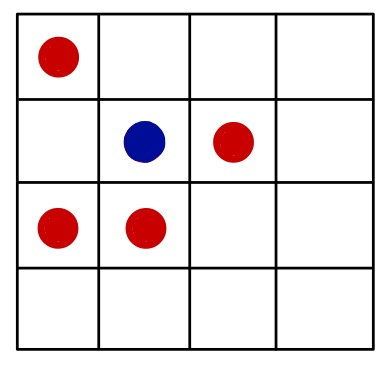
\includegraphics[height=2in]{figure/4QueensAttack.JPG}
    \caption{An attacking example of 4-queens problem: the blue queen is attacking all the red queens around it.}
    \label{fig:4queensAttack}
  \end{subfigure}%
  ~  
  \begin{subfigure}[t]{0.5\textwidth}
    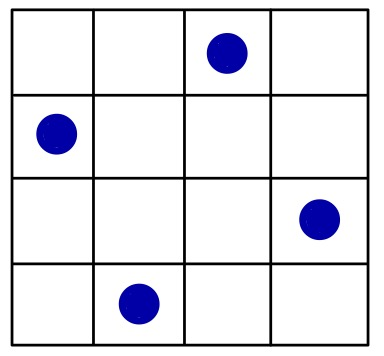
\includegraphics[height=2in]{figure/4QueensSolution.JPG}
    \caption{A solution of 4-queens problem}
    \label{fig:4queensSolution}
  \end{subfigure}%
  \caption{4-queens problem}
\end{figure}

The most famous example of N-queens problem is the eight queens puzzle, since it was first published back to early 1900s~\cite{ball_mathematical_1914}. All of its solutions can be found on Wikipedia~\cite{noauthor_eight_2017}. In next section, I will talk about some existing solutions of the N-queens problem.

\subsection{Existing results}
There are two options of finding the solutions of N-queens problem: find one solution and find all the solutions. The first one will terminate the algorithm as long as it find one valid solution and report it,  but the second one will continue search untill it find all the solutions for that problem and report all the solutions as well as the number of the solutions. It is easy to imagine that, the first one is easier than the second option. Some works only focus on finding just one solution, and they can solve the problem with a very large  $n$ (e.g. $500,000$) ~\cite{sosic_polynomial_1990}. However, the reason for these algorithms of finding just one solution is that they always use some more efficient ways to get the answer with much less time, and these efficient ways are not always guarenteed to give an answer at the end (not sound) ~\cite{sosic_polynomial_1990}. If they use a method that is garenteed to provide a solution, they can just run the algorithms multiple times to get all the solutions.

In this report, my goal is to find the existing most efficient (in terms of time performance) algorighm of solving the N-queens puzzle. The algorithm should report all the valid solutions along with the number of them. The most recent existing result of N-queens puzzle only reports the solutions up to $n=27$ (see Table~\ref{tab:numberOfSolutions}. The source of data is from the ``The On-Line Encyclopedia of Integer Sequences (OEIS)'' ~\cite{noauthor_a002562_nodate}~\cite{noauthor_a000170_nodate}. Fudamental solutions are the ones after filtering the mirrored ones of all the solutions.)

\begin{table}[]
  \centering
  \caption{Number of solutions of N-queens puzzle.}
  \label{tab:numberOfSolutions}
  \resizebox{\textwidth}{!}{%
    \begin{tabular}{|c|l|l|l|l|l|l|l|l|l|l|l|}
    \hline
    \textbf{n}                                                     & \multicolumn{1}{c|}{\textbf{1}} & \multicolumn{1}{c|}{\textbf{2}} & \multicolumn{1}{c|}{\textbf{3}} & \multicolumn{1}{c|}{\textbf{4}} & \multicolumn{1}{c|}{\textbf{5}} & \multicolumn{1}{c|}{\textbf{6}} & \multicolumn{1}{c|}{\textbf{7}} & \multicolumn{1}{c|}{\textbf{...}} & \multicolumn{1}{c|}{\textbf{25}} & \multicolumn{1}{c|}{\textbf{26}} & \multicolumn{1}{c|}{\textbf{27}} \\ \hline
    \multicolumn{1}{|l|}{\textbf{fundamental}} & 1                               & 0                               & 0                               & 1                               & 2                               & 1                               & 6                               & ...                               & 275,986,683,743,434              & 2,789,712,466,510,289            & 29,363,791,967,678,199           \\ \hline
    \textbf{all}                               & 1                               & 0                               & 0                               & 2                               & 10                              & 4                               & 40                              & ...                             & 2,207,893,435,808,352         & 22,317,699,616,364,044	   & 234,907,967,154,122,528           \\ \hline
  \end{tabular}}
\end{table}

\section{Solutions}
\subsection{Naive algorithm}
The naive way of solving N-queens puzzle is to enumerate all the possible configurations to find the right ones. This indeed is time as well as memory consuming when $n$ increase. One simple way of optimization is, instead of generating all the configurations, only gernerating the configurations that for each column or each row there is only one queen. Still the time of finishing the whole process is going to be unacceptable.

\subsection{Backtracking with CSP}\label{sec:csp}
In stead of generating all the configurations and then iterate over them to find the valid answers, we put a new queen onto the current board and check whether it will attack the existing queens that are already on the board. If it is yes, then we take that queen off and try another position. If it is no, we leave the queen in that position and pick another queen that is not on board currently as the new queen and repeat the process. Another thing we need to do is to remember all the actions we did, and if we found that there is no positions allow a new queen to be placed in, then it is time to reverse the previous process, i.e. take off the last placed queen before the current one, and then try to place it somewhere else. This process essentially is doing the depth first search on a tree. Each node on the tree is a configuration and the edges are the actions taken on the parent node and the child nodes are the result. The search process is called backtracking ~\cite{russell_modern_1995}, since it will search down and if it find a unrealized path it will backtrack to the parent nodes. Figure ~\ref{fig:backtrack4Queens} is an example of backtracking on the 4-queens puzzle.
\begin{figure}[ht]
  \centering
  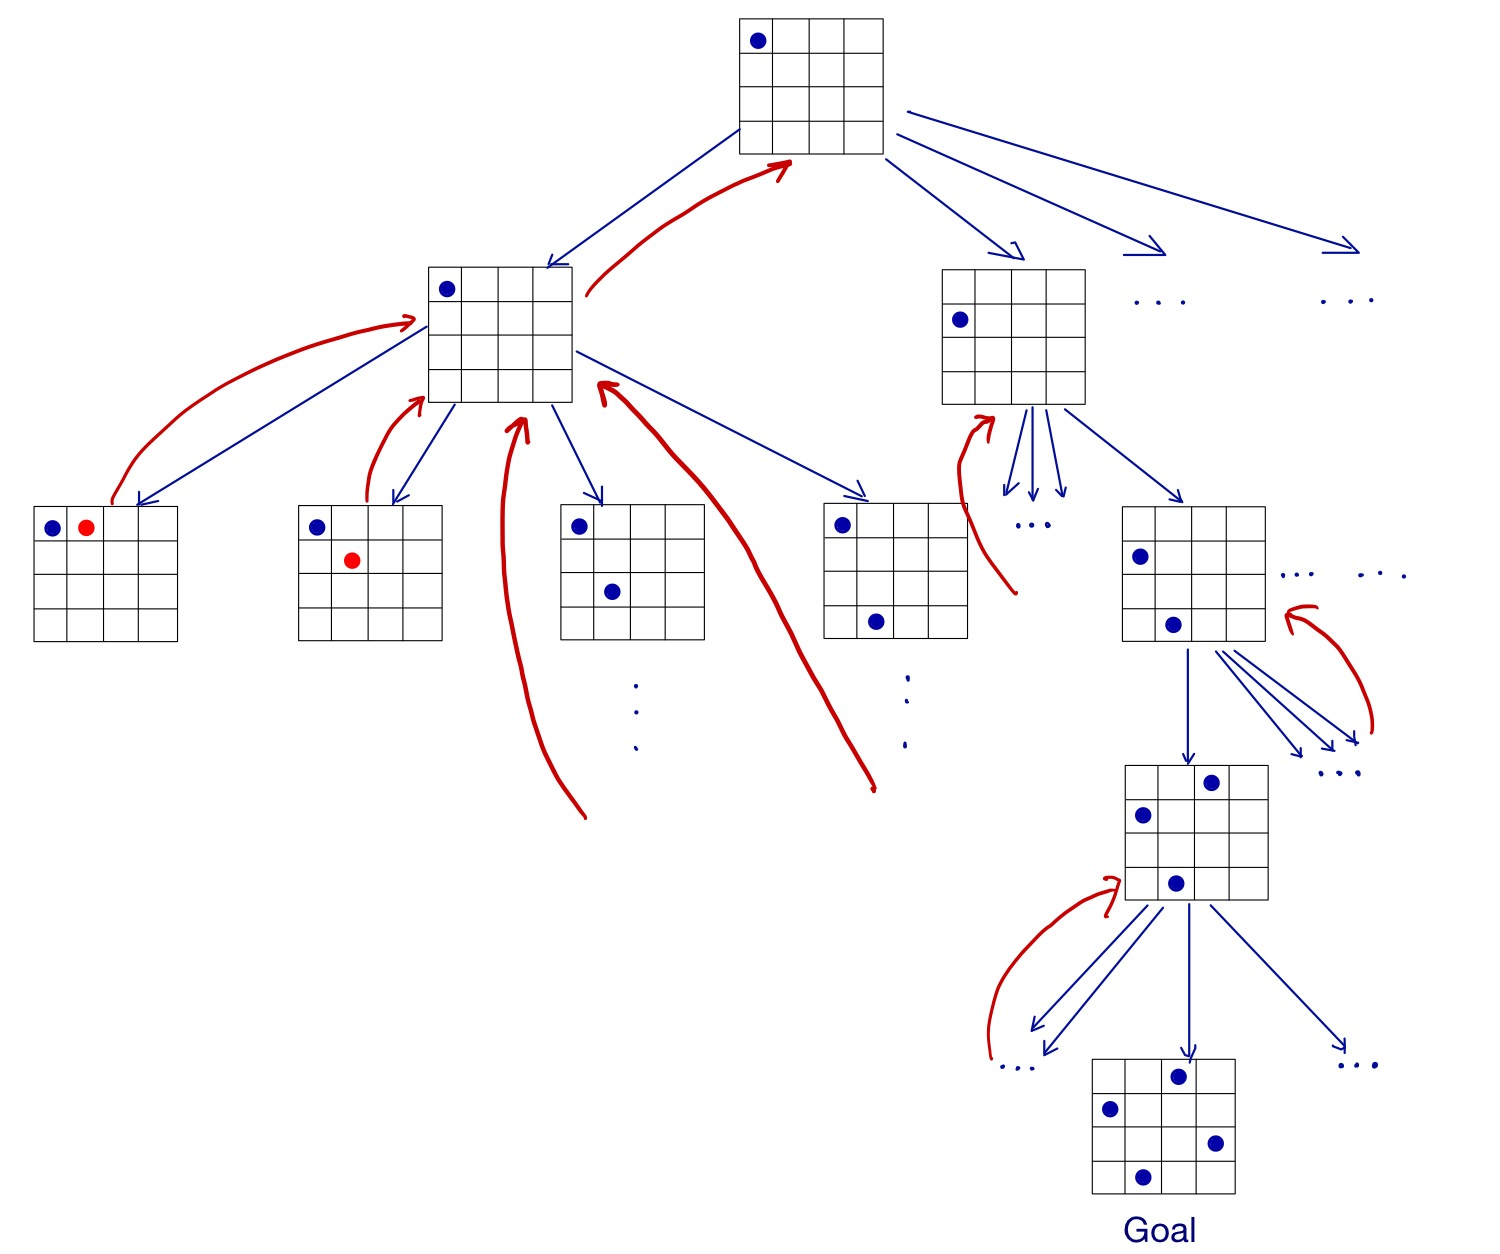
\includegraphics[width=0.8\textwidth]{figure/backtracking4Queens.JPG}
  \caption{An example of backtracking process (incomplete) for 4-queens puzzle. Each node is a configuration. The red lines indicate the backtrack actions.}
  \label{fig:backtrack4Queens}
\end{figure}


In addition, instead of looking at every queen in the configuration and do the computation every time, we need to build some data structures to help us to check the attacking condition by simply scanning the data structures. This is called constraint guided search ~\cite{russell_modern_1995}. Everytime we take an action, it must statisfy the constraint, and here the constraint is no queens stay on the same columns, rows, or diagnols. The constraint satisfication problem is shorted for CSP. In my implementation, there is an array of bits (each element's value is $0$ or $1$) to record, for every column, row and diagnol, whether there is a queen already been placed. The array's size is determined by the number $n$: the number of columns and rows are both $n$, and the number of two diaganols are both $2n-1$, so the total number is $4n-2$.

In my implementation, there is a global array for the CSP, and it does the search rescursively. Before querying a child node, it will remember the action that is going to be taken, and after  the querying is done it will reverse the actions that were taken. More details of the implementaion will be dicussed in the evaluation section. 

\subsection{Algorithm X}
Backtracking is the good way of searching process, however because the representation of each node that the backtracking works on is not good enough, the depth as well as the number of branching of the search tree is very large. This will make the searching time longer, because there are too many nodes will be traversed.

In this section, we will discuss another technque that can reform the N-queens problem into \textbf{exact cover problem} ~\cite{noauthor_exact_2017} which can make the depth and branching number much smaller. A very efficient search algorithm called \textbf{Alogrithm X}   shorted for DLX combined with another techque called \textbf{Dancing Links alorithm} ~\cite{noauthor_knuths_2016}~\cite{knuth_dancing_2000} is used, the search tree is going to be much smaller. Here I am going to expain what the exact cover problem is, how we convert the N-queens problem to exact cover problem, and how the dancing links works in Algorithm X. Therefore, we can first convert our problem into Exact Cover problem and use Algorithm X to solve it fast.

\subsubsection{Exact cover problem}
Exact cover problem is defined like this: given a set $X$, and a collection $S$ of $X$'s subsets, the goal is to find another collection $S^*$ in which every subset $y$ is in $S$ and dose not intersect with other subset, as well as the union of all the subset in $S^*$ is exactly set $X$. Here we use an example to explain it. Suppose $X={1,2,3,4,5,6}, S={A, B, C, D, E}, A={1,3}, B={2,4, 5}, C={1, 6}, D={3},E={1, 3, 6}$, then the $S^*$ should be $S^*={B, E}$. We can use the a matrix to represent this example (see Figure~\ref{fig:ecp}.)

\begin{figure}[ht]
  \centering
  \begin{subfigure}[t]{0.5\textwidth}
    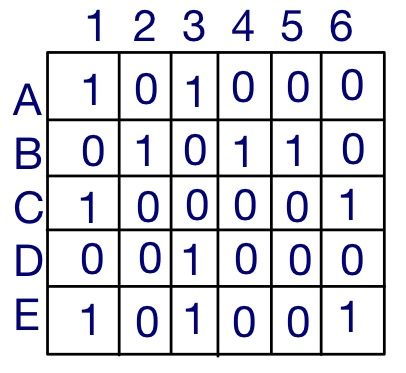
\includegraphics[height=1.5in]{figure/ecp_1.JPG}
    \caption{One matrix representation of an example of the exact cover problem.}
    \label{fig:ecp_1}
  \end{subfigure}%
  ~  
  \begin{subfigure}[t]{0.5\textwidth}
    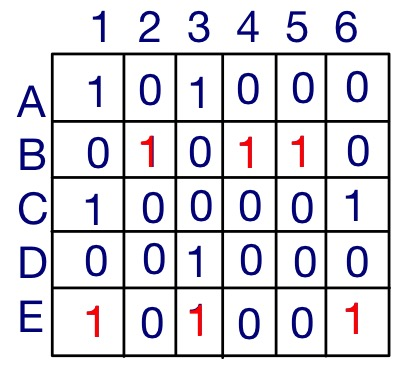
\includegraphics[height=1.5in]{figure/ecp_2.JPG}
    \caption{A solution of the example. Every column has only one red $1$s when we choose $B$ and $E$ as the solution. }
    \label{fig:ecp_2}
  \end{subfigure}%
  \caption{An example of exact cover problem}
  \label{fig:ecp}
\end{figure}

The good way to solve exact cover problem  is to Algorithm X. It wil first count the number of $1$s in each column, and then pick the leftmost column with number of $1$s larger than zero. Then \textbf{cover} (see Figure ~\ref{fig:algorithmX}) this column and record this operation. After covering this column, the matrix's size is dramatically reduced (see Figure ~\ref{fig:algorithmX}). Then repeat this process recursively. If there is no columns with at least one $1$, then the search on this branch fails, and all the operations have been done have to be reversed (see Section~\ref{sec:dl}). The original algorithm X was introduced by Donald Knuth in his paper called \textit{Dancing links} ~\cite{knuth_dancing_2000}, and below is the algorithm we quote from that paper:

\begin{quotation}
  If $A$ is empty, the problem is solved; terminate successfully.
  
  Otherwise choose a column, $c$ (deterministically).
  
  Choose a row, $r$, such that $A[r, c] = 1$ (nondeterministically).
  
  Include $r$ in the partial solution.
  
  For each $j$ such that $A[r, j] = 1$,
  
  \indent \indent  delete column $j$ from matrix $A$;
  
  \indent \indent  for each $i$ such that $A[i, j] = 1$,
  
  \indent \indent \indent     delete row $i$ from matrix $A$.
  
  Repeat this algorithm recursively on the reduced matrix $A$.
\end{quotation}

\subsubsection{Conver N-queens to exact cover problem}
If we think about the array we mentioned in Section~\ref{sec:csp} again, we can notice that each element of the array can only have one $1$. That is exactly the columns mentioned before. Each row in the matrix is a position on the board. Therefore, there are $n^2$ rows. Thus, we can initialize the matrix for our exact cover problem.

\subsubsection{Dancing links}\label{sec:dl}
Because in the backtracking process, we need to reverse the operations we did, the cost of recording and reversing operations must be inexpensive. In Donald's paper~\cite{knuth_dancing_2000}, he constructed double-linked lists to represent rows and columns in the matrix. Therefore, the cost of updating and reversing is cheap. Removing one element in a double-linked list can use these two operations: $L[R[x]]\leftarrow L[x]$ and $R[L[x]]\leftarrow R[x]$. Adding back the removed element only needs two very simple operations: $L[R[x]]\leftarrow x$ and $R[L[x]]\leftarrow x$.  Therefore, we can do the search by removing the elements in the matrix from top to bottom and left to right, while adding back them from bottom to top and right to left. This whole process make the double-linked list `dance' in the matrix, so it is called dancing links.

\subsection{DLX with heuristic}

\subsection{Other algorithms}

\section{Evaluation}

\section{Conclusion}

\section{Future work}


\bibliography{report-ref}{}
\bibliographystyle{acm}


\end{document}
